\documentclass{report}
\usepackage{ptext}
\usepackage{lipsum}
\usepackage{graphicx}
\usepackage{ptext}

\input{Boostan-UserManual}

\newword{Abstraction}{Abstraction}
{انتزاع}{}

\newword{Abstract}{Abstract}
{انتزاعی}{}

\newword{AbsoluteMinimum}{Absolute Minimum}
{کمینه مطلق}{}


\newword{AcceptableCell}{Acceptable Cell}
{سلول پذیرفتنی}{سلول‌های پذیرفتنی}

\newword{AccessBurst}{Access Burst}
{توده دسترسی}{توده‌های دسترسی}


%%% S
\newword{Sample}{Sample}
{نمونه}{نمونه‌ها}

\newword{SamplePath}{Sample Path}
{نمونه مسیر}{}

\newword{SampleSpace}{Sample Space}
{فضای نمونه}{فضای نمونه‌ها}
\newacronym{ACK}{ACK}{Acknowledgement}

\newacronym{ACI}{ACI}{Application Control Interface}

\newacronym{ACIR}{ACIR}{Adjacent Channel Interference Ratio}

\newacronym{ACLC}{ACLC}{Adaptive Configuration of Logical Channels}

\newacronym{ACLP}{ACLP}{Adjacent Channel Leakage Power}

\title{مستند راه اندازی پروژه نهایی درس شبکه های تلفن همراه}
\type{مستند }
\author{زهرا دهقان\\اسماء حمید\\فاطمه شرح دهی مقدم}

\logofile{Pic/logo}


\begin{document}

\pagenumbering{gobble}
\Godpage
\maketitle
\pagenumbering{arabic}
\tableofcontents


\chapter{\lr{Polaris Server}}

برای راه‌اندازی \lr{Polaris Server}، ابتدا با دستور زیر یک \lr{Virtual Environment} بسازید:

\begin{lstlisting}[language=bash]
python -m venv venv
\end{lstlisting}

سپس با استفاده از دستور زیر تمامی پکیج‌های مورد نیاز را نصب کنید:

\begin{lstlisting}[language=bash]
pip install -r requirements.txt
\end{lstlisting}

برای اجرای برنامه، از دستور زیر استفاده کنید:

\begin{lstlisting}[language=bash]
python manage.py runserver 0.0.0.0:8000
\end{lstlisting}

برای ایجاد یک ادمین، از دستور زیر استفاده کنید:

\begin{lstlisting}[language=bash]
python manage.py createsuperuser
\end{lstlisting}


\chapter{ \lr{Web Application}}
\section{ورود به سامانه}
برای ورود به سامانه و استفاده از داشبورد کاربری شخص خودتان ، در صفحه ورود شماره همراه و رمزی که در اپلیکشن Polaris ست کرده بودید را وارد کنید. بعد ازین مرحله وارد داشبورد کاربری خود می‌شوید.
\begin{figure}[ht]
	\centering
	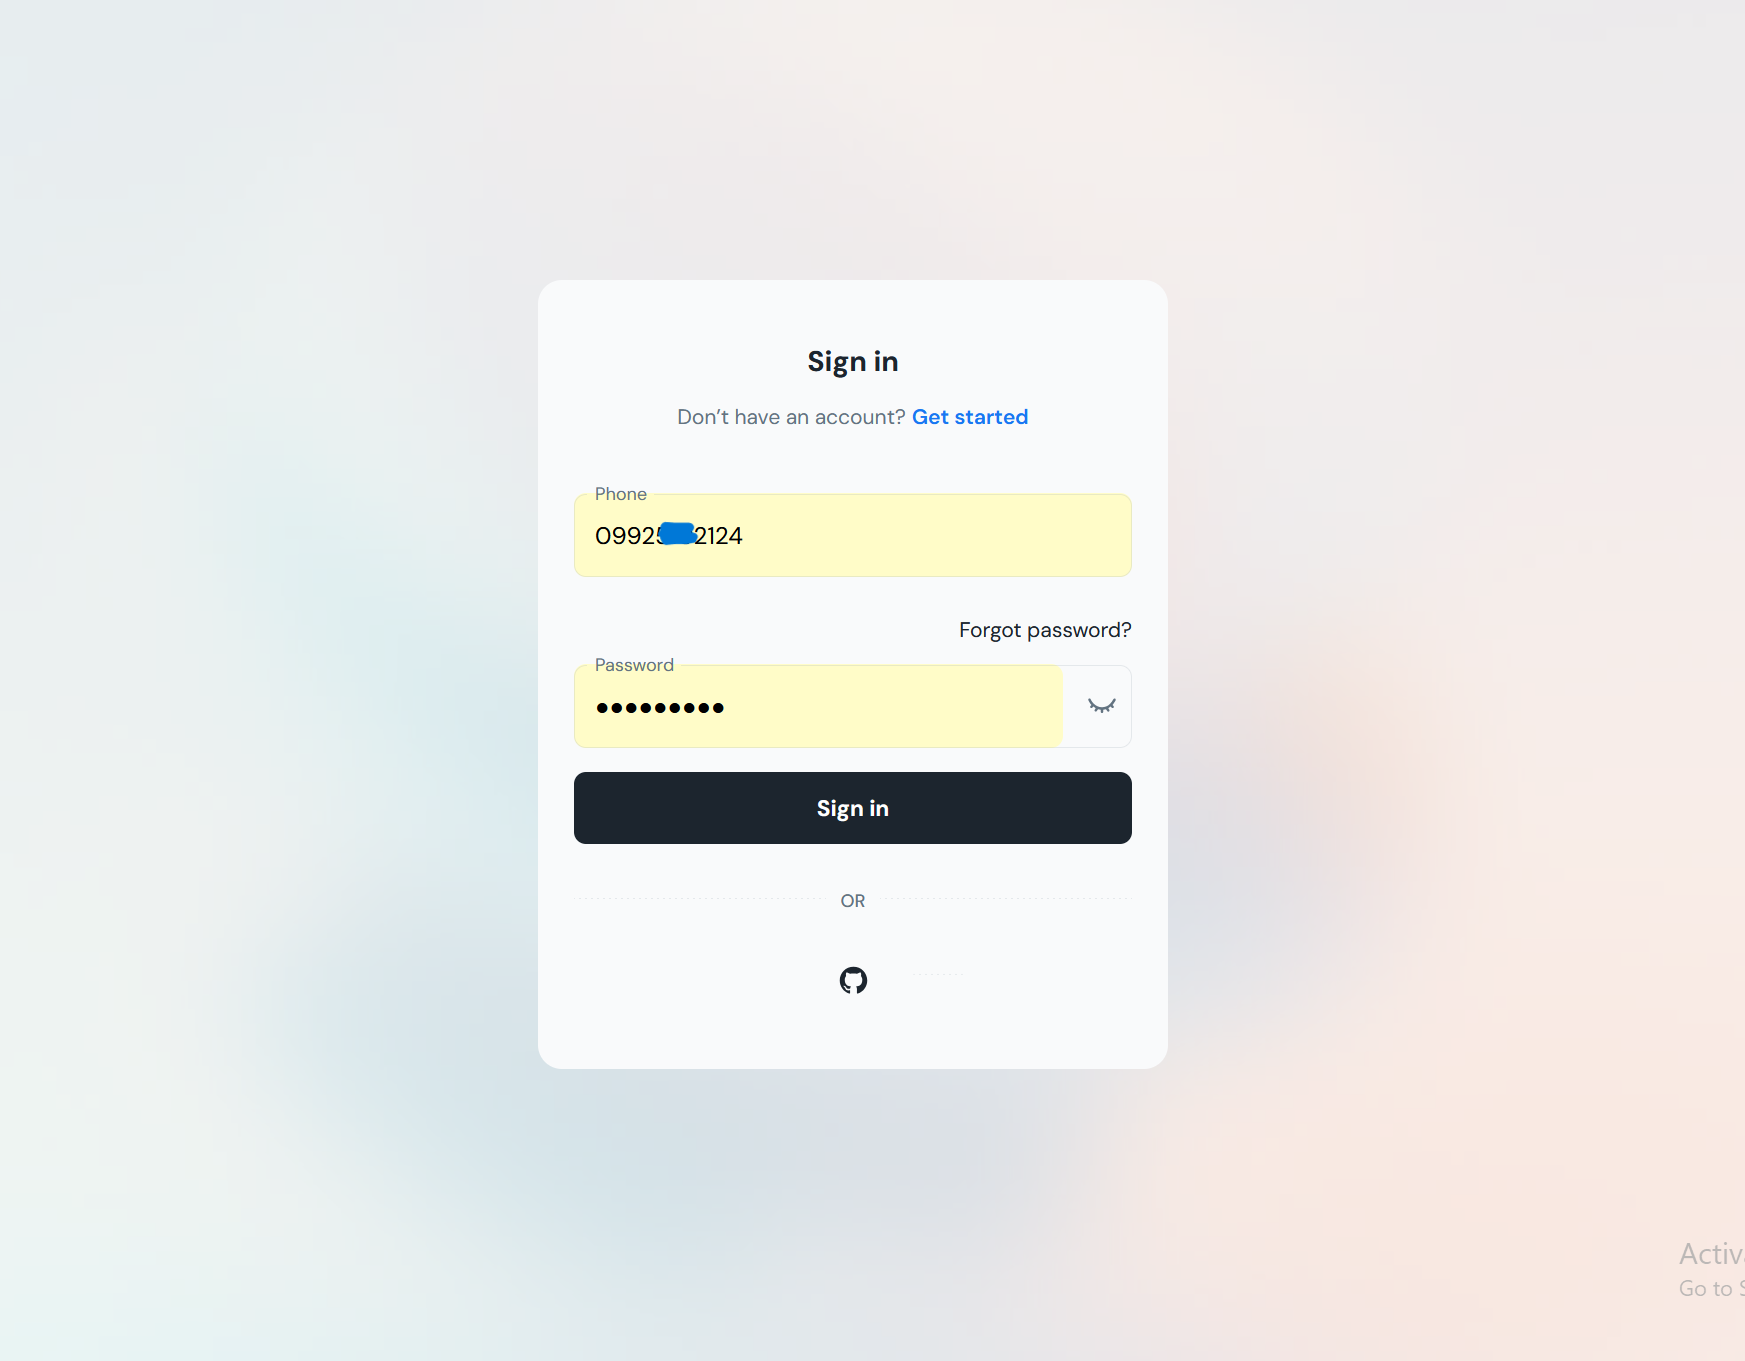
\includegraphics[width=0.7\textwidth,height=10cm,keepaspectratio]{Pic/signup_front}
	\caption{ورود}
	\label{fig:signup_front}
\end{figure}
\section{Sidebar}
در نوار کناری سامانه Polaris گزینه‌هایی وجود دارند که به شما این امکان را می‌دهند که دسترسی راحتی به امکانات موجود در سامانه داشته باشید.
در ادامه به ارائه اطلاعاتی در رابطه با هر ویژگی سامانه می‌پردازیم.
  \begin{figure}[ht]
	\centering
	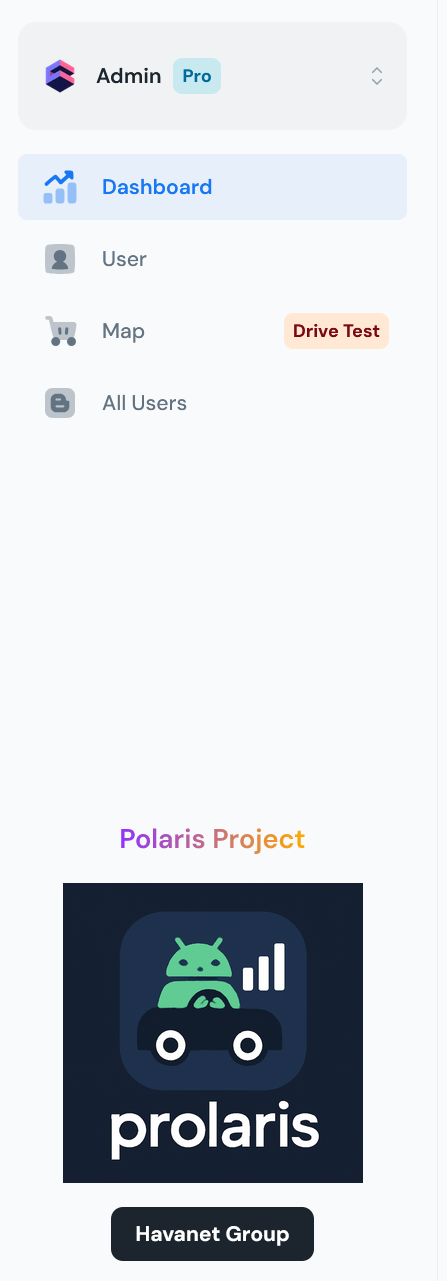
\includegraphics[width=0.7\textwidth,height=10cm,keepaspectratio]{Pic/sidebar}
	\caption{Sidebar}
	\label{fig:sidebar}
\end{figure}
\section{داشبورد}
در این صفحه شما دسترسی به تمامی اطلاعات و تجزیه و تحلیل‌های شبکه خواهید داشت. در داشبورد سامانه Polaris شما کارت‌های مختلفی مشاهده خواهید کرد که هر کدام به صورت اختصاصی به نمایش تحلیل نتایج داده تست‌های شما که در اپلیکیشن انجام دادید می‌پردازند. تست‌های نمایش داده شده شامل نتایج \textbf{dns}, \textbf{ping}, \textbf{web response time}, \textbf{upload/download rate} و \textbf{تست پیامک} هستند.
 \begin{figure}[ht]
	\centering
	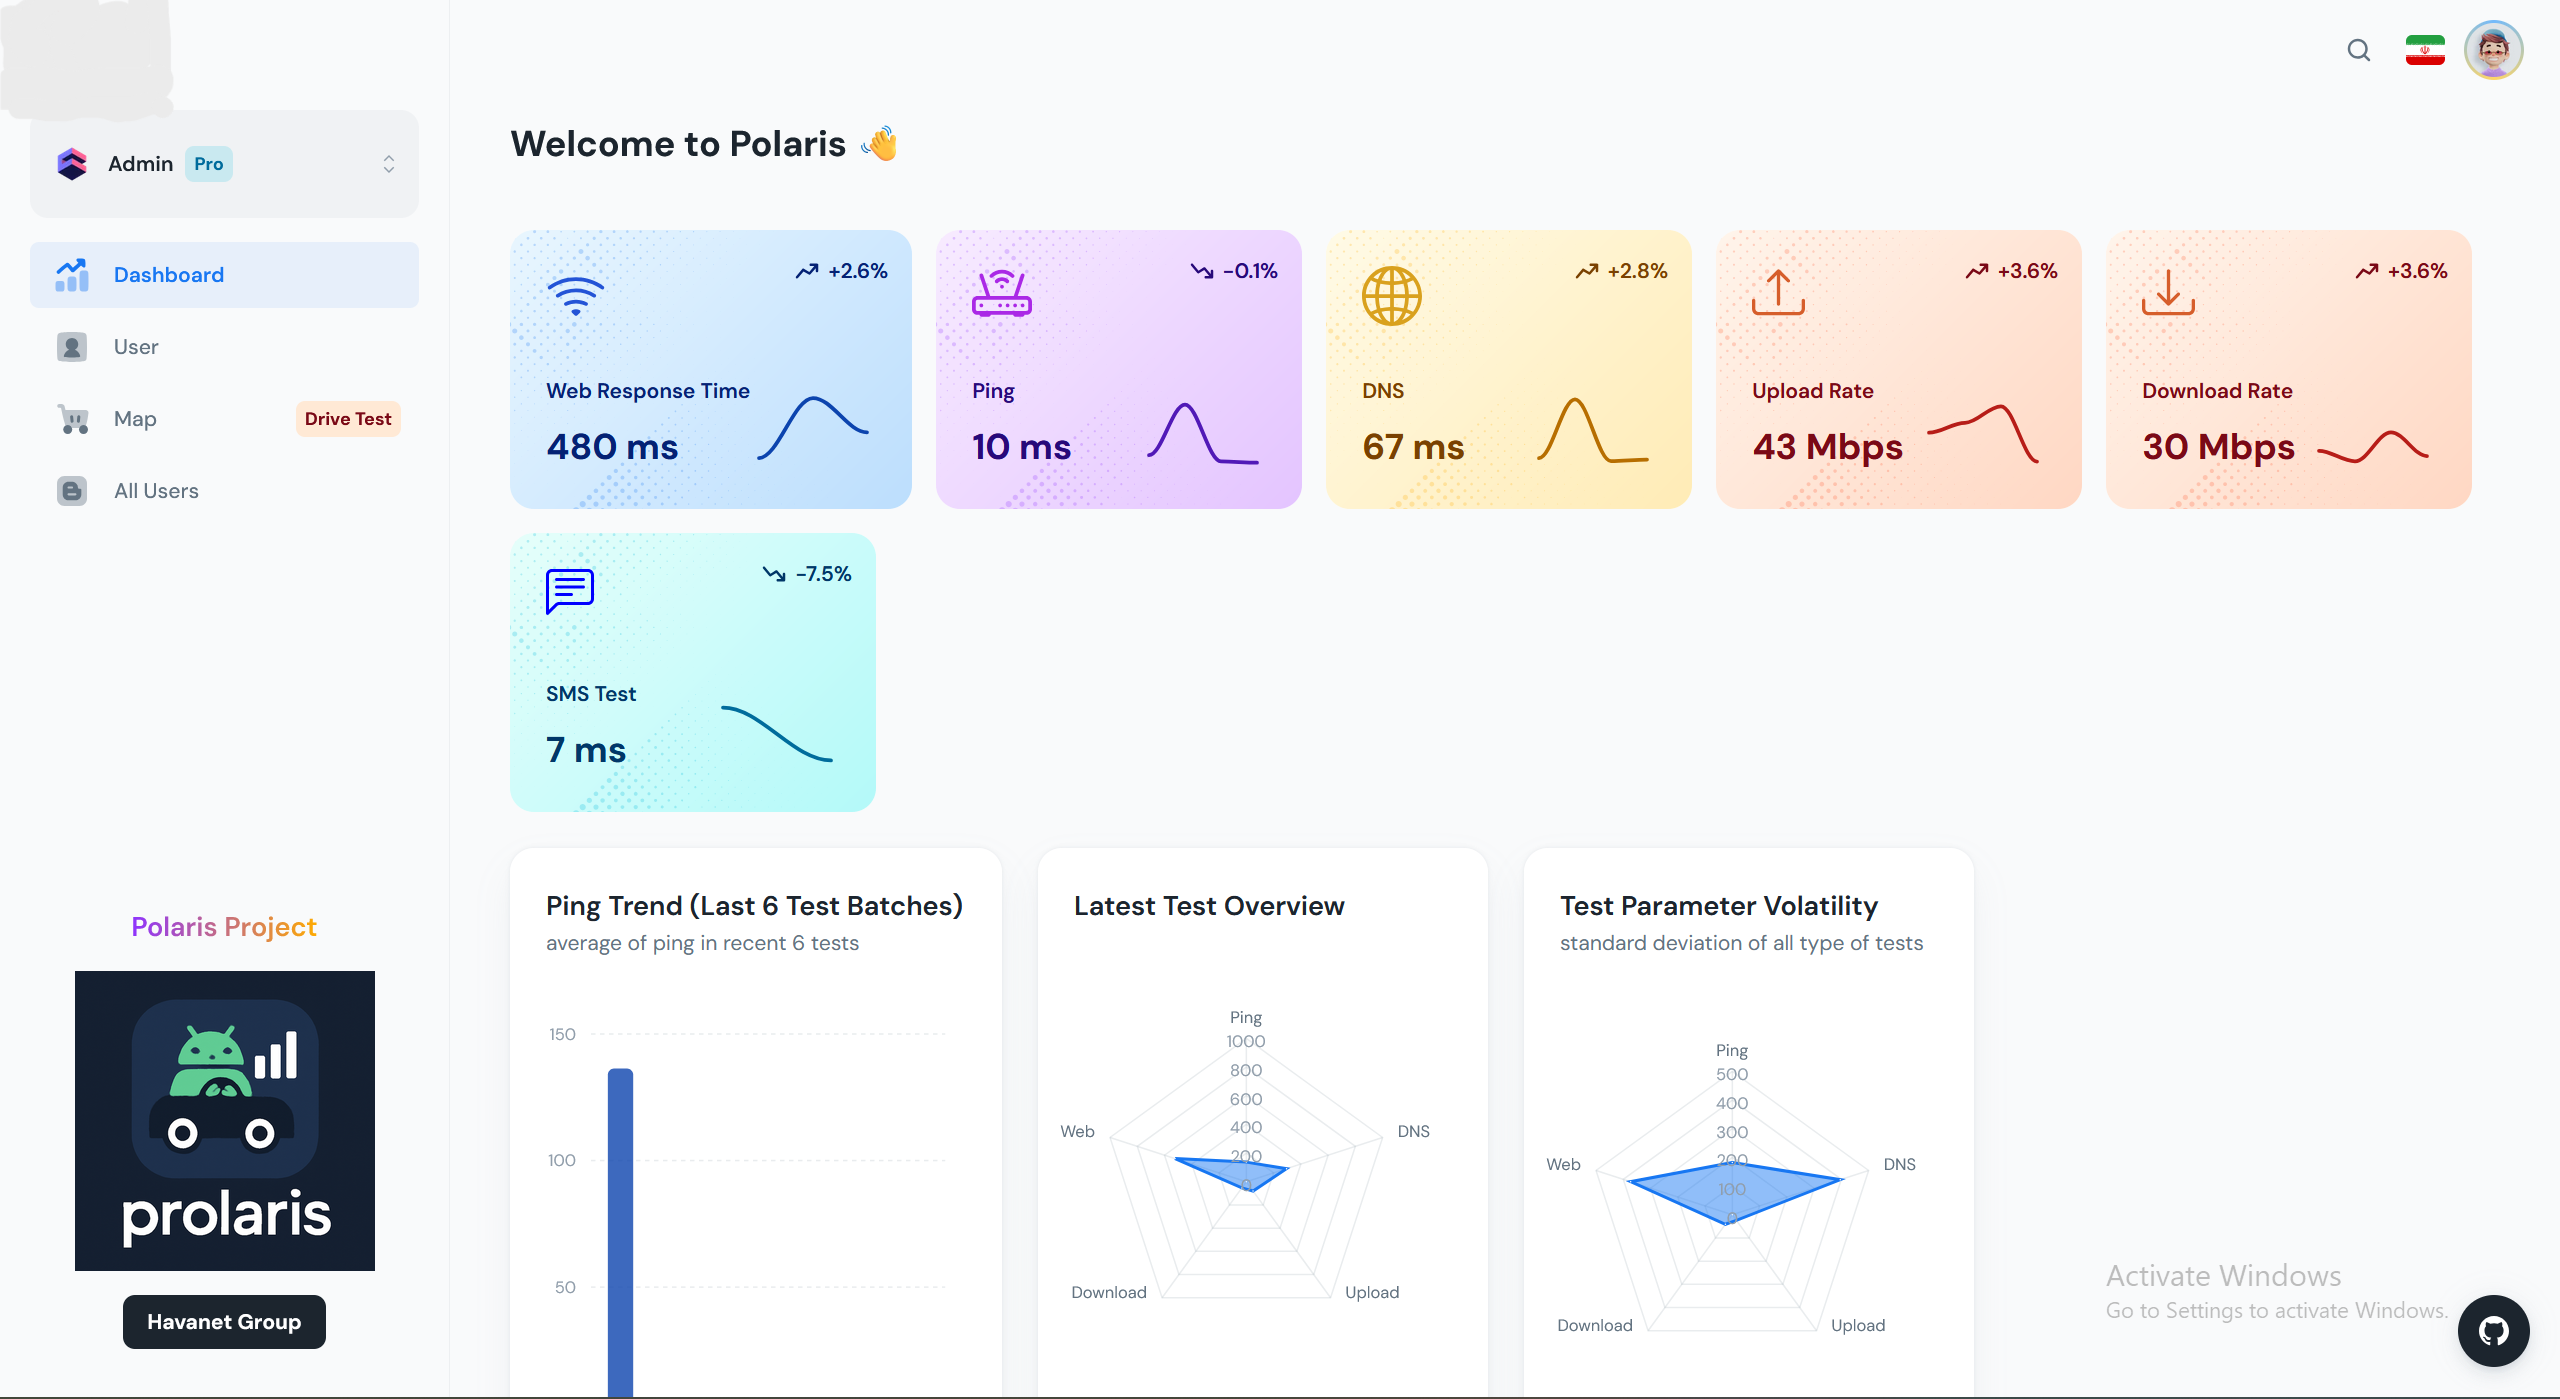
\includegraphics[width=0.7\textwidth,height=10cm,keepaspectratio]{Pic/dashboard}
	\caption{ داشبورد}
	\label{fig:dashboard}
\end{figure}

\subsection{نحوه کسب اطلاعات در رابطه با نتایج تست‌ها}
هر 6 پارامتر تست شده در اپلیکیشن پولاریس، کارت نمایش نتیجه و تحلیل مخصوص به خودشان را دارند. برای خوانایی بیشتر و تجربه کاربری بهتر، تمپلیت هر 6 کارت یکسان است. نتیجه عددی آخرین تست گرفته شده از هر پارامتر در کارت دیده می‌شود. به علاوه، نموداری جهت نمایش روند تغییرات 12 تست اخیر در پایین سمت راست هر کارت قابل مشاهده است که با هاور کردن روی آن، نتیجه عددی تست‌ها نیز در یک کادر کوچک به شما نمایش داده می‌شود.

\subsection{دیگر نمودارهای تحلیلی}
\paragraph{روند تغییرات پینگ}
در این نمودار، برای بررسی بهتر تاریخچه تست‌های یک پارامتر و انجام تحلیل دقیق‌تری روی شبکه، نموداری با این ساختار طراحی شده است. هر 6 میله نمودار ستونی نماینده میانگین دوازده تست پشت سر هم از لحاظ زمانی می‌باشد.
 \begin{figure}[ht]
	\centering
	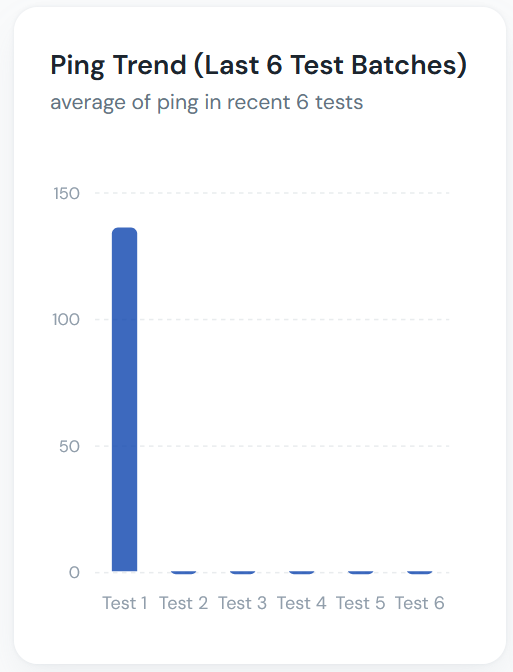
\includegraphics[width=0.7\textwidth,height=10cm,keepaspectratio]{Pic/ping}
	\caption{ نتایج تست پینگ}
	\label{fig:ping}
\end{figure}

\paragraph{Latest Test Overview نمودار}
اگر مایلید با یک نگاه کلی به کیفیت آخرین تست‌های گرفته شده خود بپردازید، این نمودار را به شما پیشنهاد می‌کنیم. این نمودار نمای کلی از وضعیت عملکرد شبکه شما در آخرین تست انجام شده را نمایش می‌دهد. هر پارامتر (مثل \textbf{Web}, \textbf{Ping}, \textbf{Download}, \textbf{DNS} و \textbf{Upload}) در بازه‌ای از 0 تا 100 درصد به نمایش گذاشته می‌شود. در اینجا هر چه مقدار بیشتر به سمت 100 درصد حرکت کند، نشان دهنده کیفیت بهتر آن پارامتر است.
 \begin{figure}[ht]
	\centering
	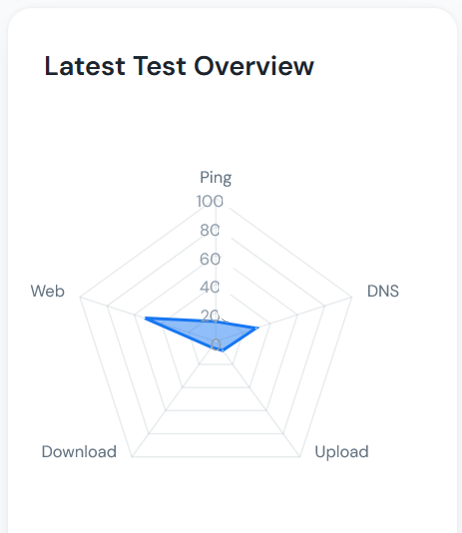
\includegraphics[width=0.7\textwidth,height=10cm,keepaspectratio]{Pic/latest}
	\caption{آخرین تست‌ها}/
	\label{fig:latest}
\end{figure}
\paragraph{Test Parameter Volatility نمودار}
برای بررسی کلی میزان نوسانات نتایج پارامترهای تست شده می‌توانید نگاهی به نمودار زیر بیندازید. مقیاس این نمودار نیز از 0 تا 100 درصد است و هر چه مقدار بیشتر به سمت 100 درصد باشد، نوسانات بیشتری در آن پارامتر مشاهده می‌شود. برای مثال، اگر مقدار \textbf{Web} در این نمودار نزدیک به 100 درصد باشد، نشان دهنده نوسانات زیاد در کیفیت وب در طول زمان است.
 \begin{figure}[h]
	\centering
	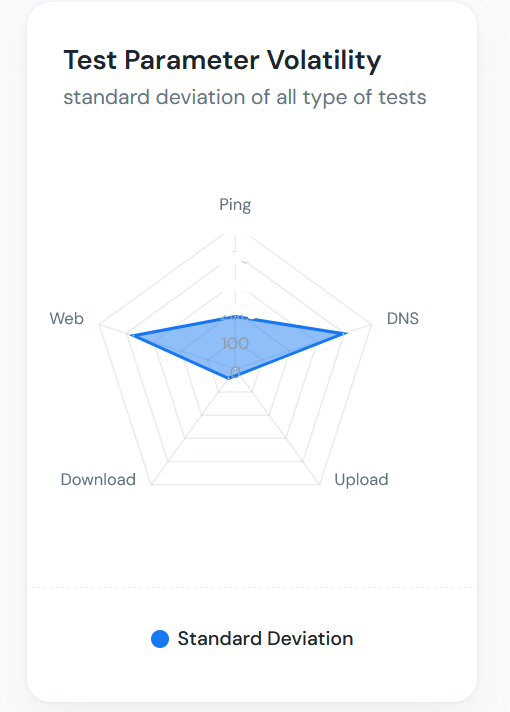
\includegraphics[width=0.7\textwidth,height=10cm,keepaspectratio]{Pic/param}
	\caption{پارامترهای تست شده}
	\label{fig:parameter}
\end{figure}
\paragraph{Download Test Qualities}
این کارت کیفیت تست‌های دانلود شما را با استفاده از سه دسته‌بندی \textbf{"MediumQ"}, \textbf{"LowQ"} و \textbf{"GoodQ"} نمایش می‌دهد. هر بخش نمایانگر درصدی از تست‌ها است که به هر کدام از این سه گروه تعلق دارند. این کارت کمک می‌کند تا کیفیت کلی دانلودها در شبکه خود را مشاهده کنید و ببینید که چه درصدی از تست‌ها به سرعت‌های پایین، متوسط یا خوب تعلق دارند.

\paragraph{Improvement Rates}
اگر به دنبال بررسی درصد بهبود پارامترها هستید، نگاهی به این نمودار بیندازید. این کارت نشان دهنده میزان بهبود در هر یک از پارامترهای تست از جمله \textbf{SMS}, \textbf{دانلود}, \textbf{آپلود}, \textbf{DNS} و \textbf{Ping} است. به عبارت دیگر، این نمودار به شما نشان می‌دهد که در مقایسه با تست قبلی، عملکرد شبکه شما در هر یک از این پارامترها به چه میزان تغییر کرده است. دقت کنید که برای هر پارامتر دو تست آخر در نظر گرفته شده‌اند که هر کدام درصد بهبود نتیجه خودشان با تست قبلی‌شان را نمایش می‌دهد.

\paragraph{News}
اگر علاقمند به دنیای تکنولوژی و شبکه‌های تلفن همراه هستید، می‌توانید تازه‌ترین اخبار منتشر شده در GSMA را در این بخش ببینید.

\paragraph{Traffic by Site}
میزان کاربرانی که مانند شما به ما اعتماد کرده و از سامانه ما استفاده می‌کنند، در این بخش به نمایش گذاشته می‌شود.

 \begin{figure}[ht]
	\centering
	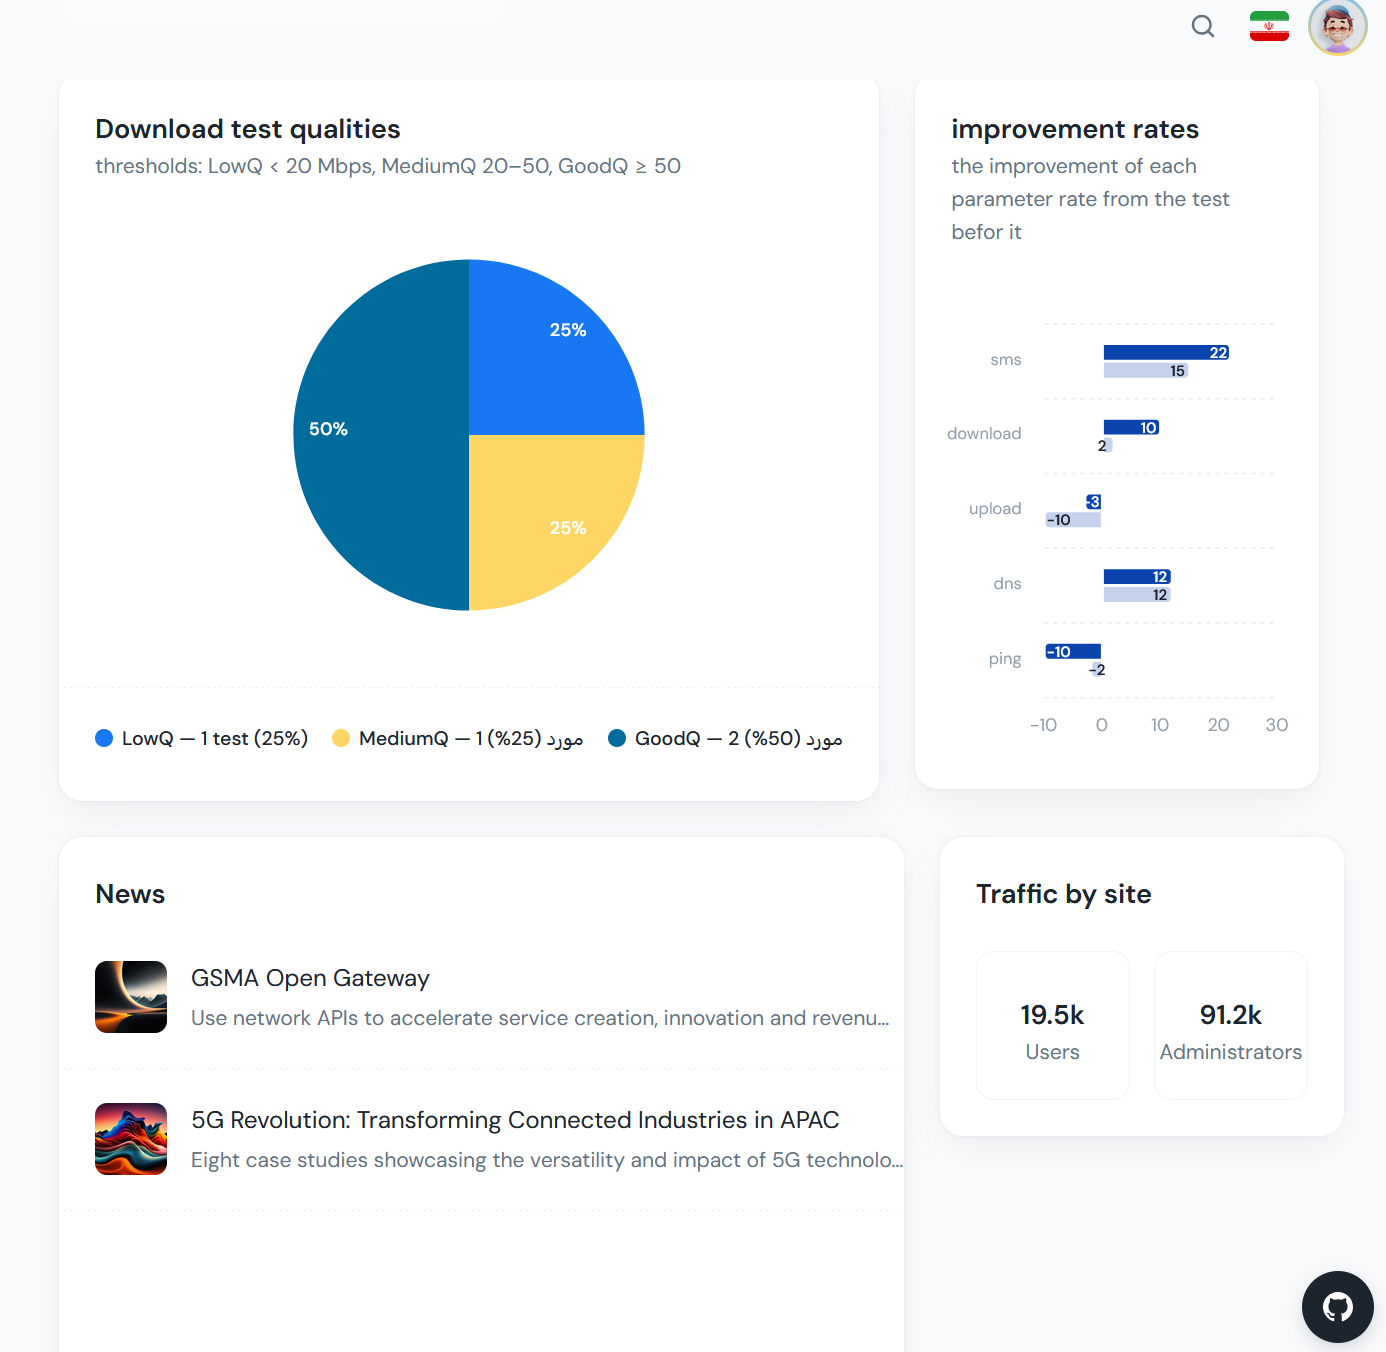
\includegraphics[width=0.7\textwidth,height=10cm,keepaspectratio]{Pic/traffic}
	\caption{ترافیک سایت ، اخبار ، نمودار بهبود و نمودار دایره ای پارامتر}
	\label{fig:traffic}
\end{figure}
\section{جدول نتایج}
برای گزارش برخط تمامی سیگنال‌های دریافتی هنگام تست، این جدول طراحی شده تا تمام ویژگی‌ها و شاخص‌های سیگنال نتیجه را گزارش کند. هر ردیف نمایانگر اطلاعات یک رکورد دیتابیس یا همان سیگنال است و هر ستون به یک ویژگی اشاره دارد.
قابلیت فیلتر نتایج نیز در نظر گرفته شده تا امکان تحلیل دقیق‌تر و سریع‌تر را به شما بدهد. شما می‌توانید فیلتر خود را بر اساس پارامترهای خاص، نسل‌های مشخص و تکنولوژی‌های مد نظر خود اعمال کنید.
در نهایت، اگر فیلتر مد نظر شما در گزینه‌های پیشنهادی نبود، باکس سرچی برای شما تعبیه شده است که هر نوع عبارت دلخواه خود که ممکن است در جدول وجود داشته باشد را بیابید. امکان انتخاب یک ردیف یا ردیف‌های متوالی برای پاک کردن آنها از جدول را نیز دارید.
\\
در نهایت اگر فیلتر مد نظر شما در گزینه های پیشنهادی نبود باکس سرچی برای شما تعبیه کردیم که هر نوع عبارت دلخواه خود که ممکن است در جدول وجود داشته باشد را بیابید.
امکان انتخاب یک ردیف یا ردیف های متوالی برای پاک کردن آنها از جدول را نیز دارید.
با کلیک بر روی دکمه دانلود اکسل شما میتوانید از کل جدول خروجی اکسل دریافت کنید .
با انتخاب ردیف مد نظر خود و کلیک بر دکمه دانلود خروجی kml  مدنظرتان را جهت باز کردن در google earth دریافت میکنید.
جدول قابلیت اسکرول کردن دارد و باقی ستون ها را میتوانید ببینید.
میتوانید جدول خود را با استفاده از علامت فلش رو به بالا یا پایین به ترتیب زمان صعودی یا نزولی مرتب کنید.
\begin{figure}[!htbp]
	\centering
	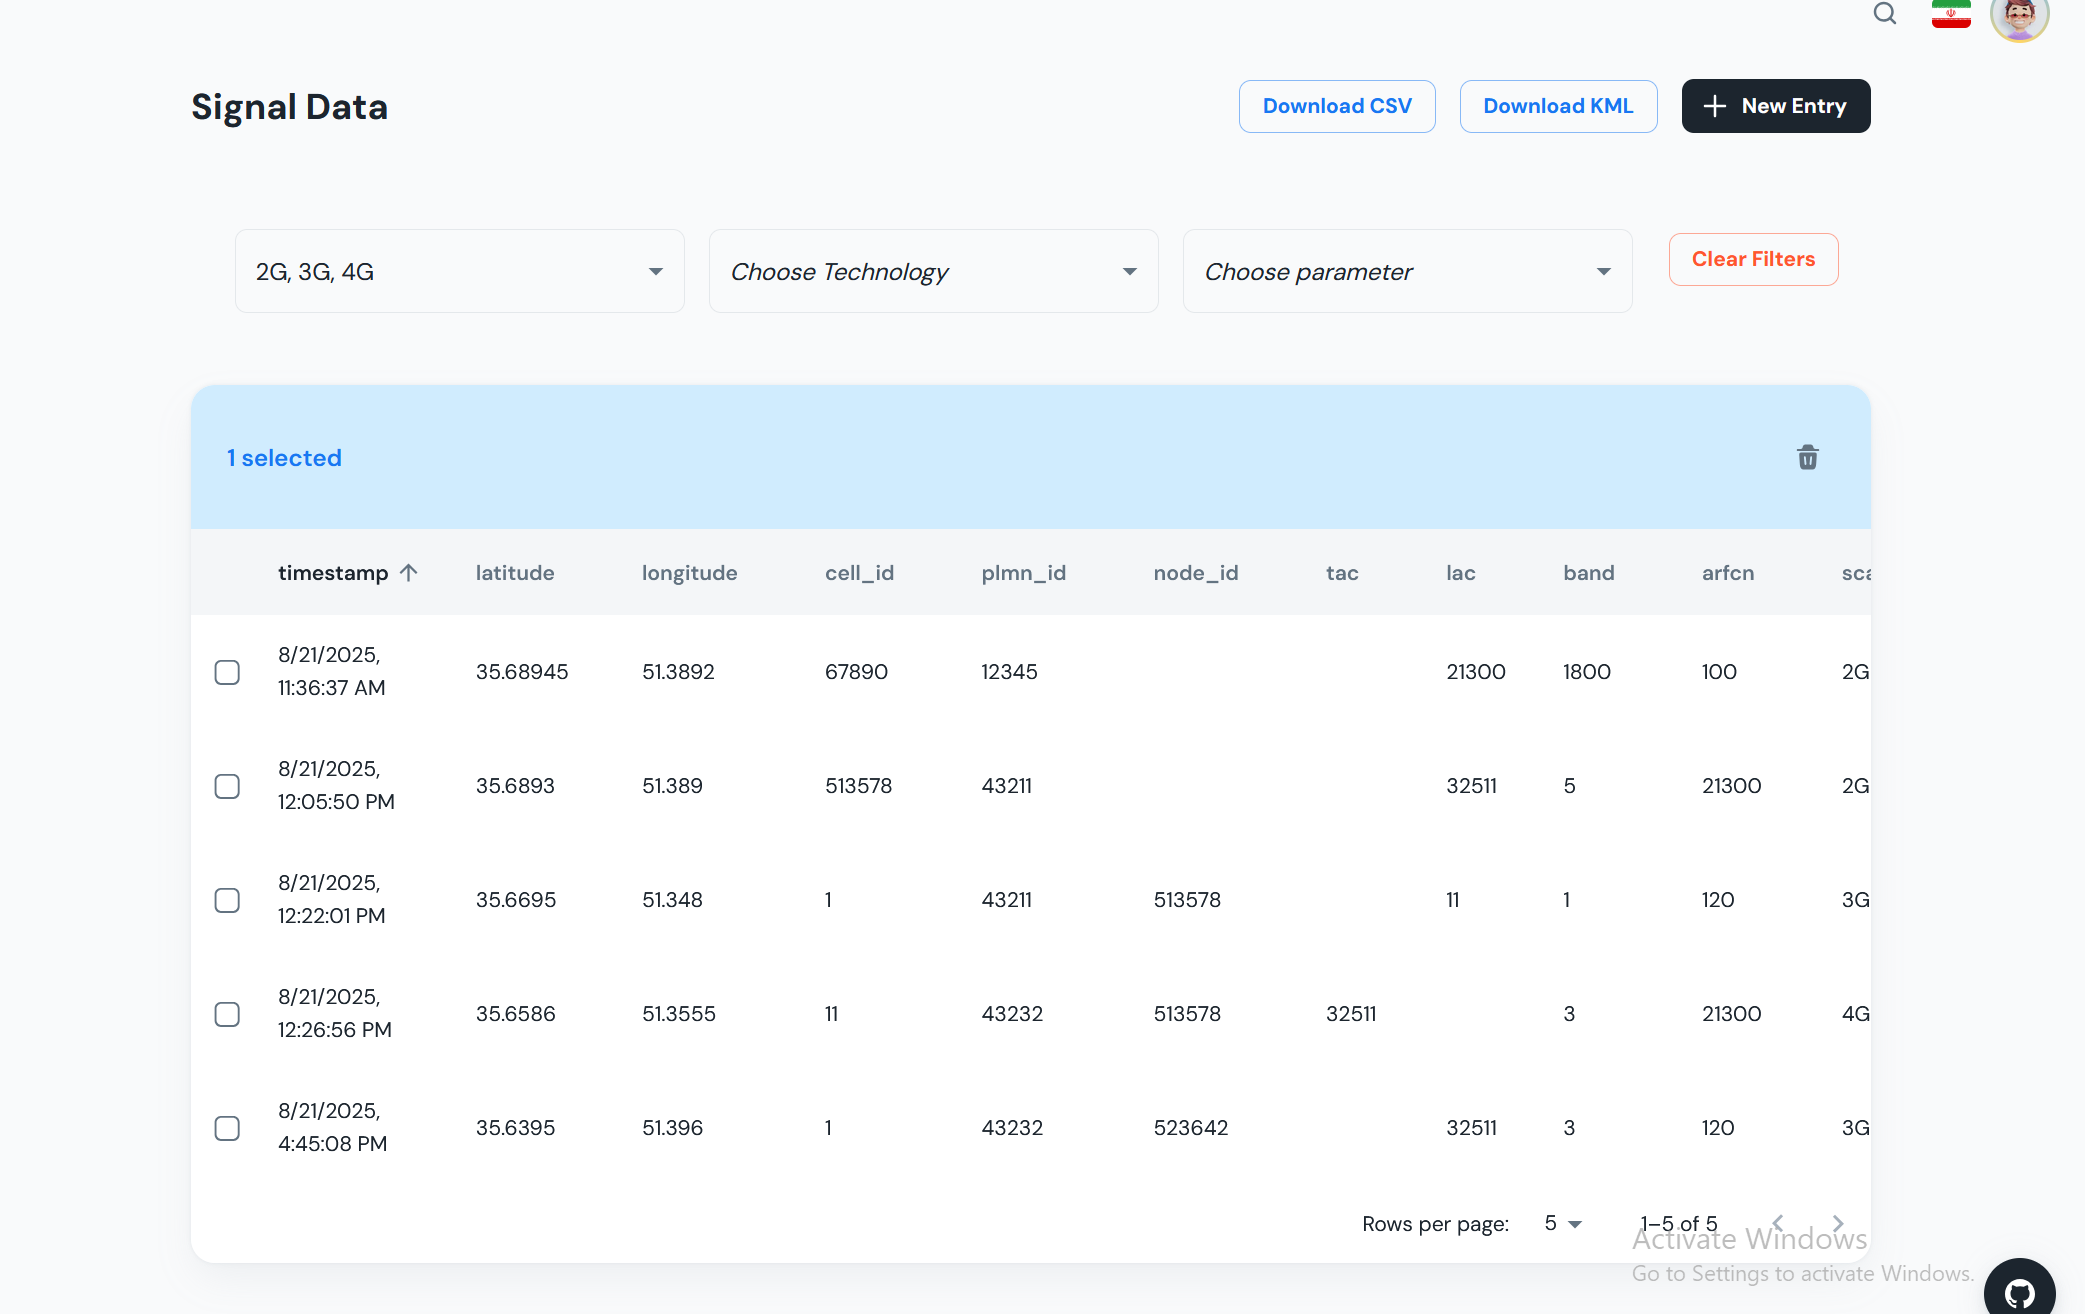
\includegraphics[width=0.7\textwidth,height=10cm,keepaspectratio]{Pic/final_table}
	\caption{جدول نتایج}
	\label{fig:table}
\end{figure}

\section{نقشه}
در این بخش، شما می‌توانید اطلاعات موقعیتی مربوط به شبکه را مشاهده کنید. این ابزار به شما امکان می‌دهد که داده‌های مربوط به تست‌های شبکه موبایل و نتایج آنها را بر اساس موقعیت جغرافیایی روی نقشه ببینید.
\begin{figure}[h]
	\centering
	\begin{subfigure}[b]{0.4\textwidth}\centering
		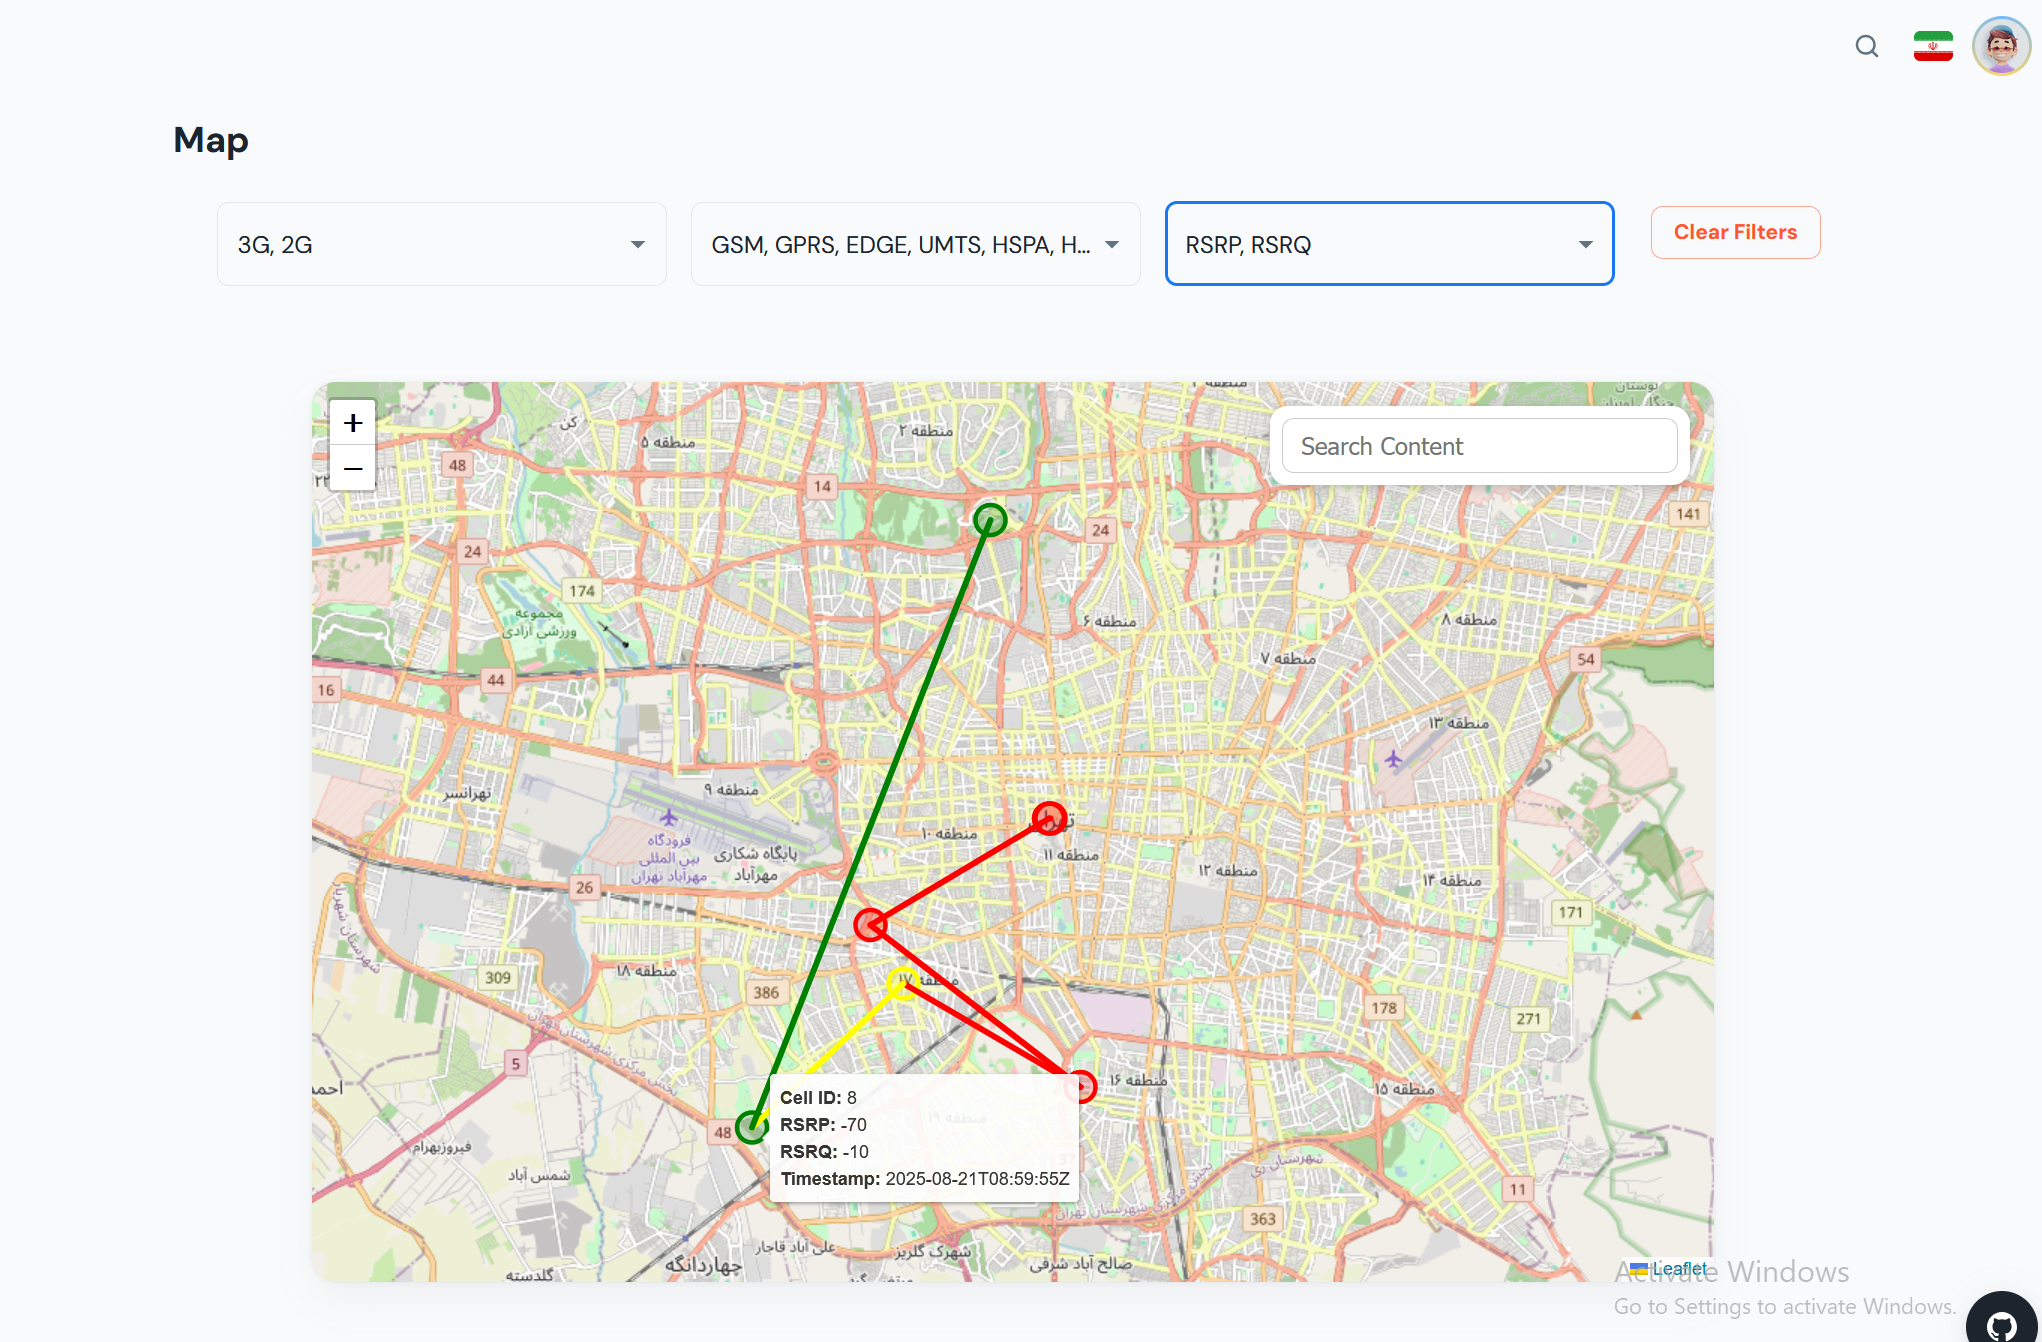
\includegraphics[width=0.7\textwidth,height=15cm,keepaspectratio]{Pic/map}
		\label{fig:map}
	\end{subfigure}
	\begin{subfigure}[b]{0.4\textwidth}\centering
		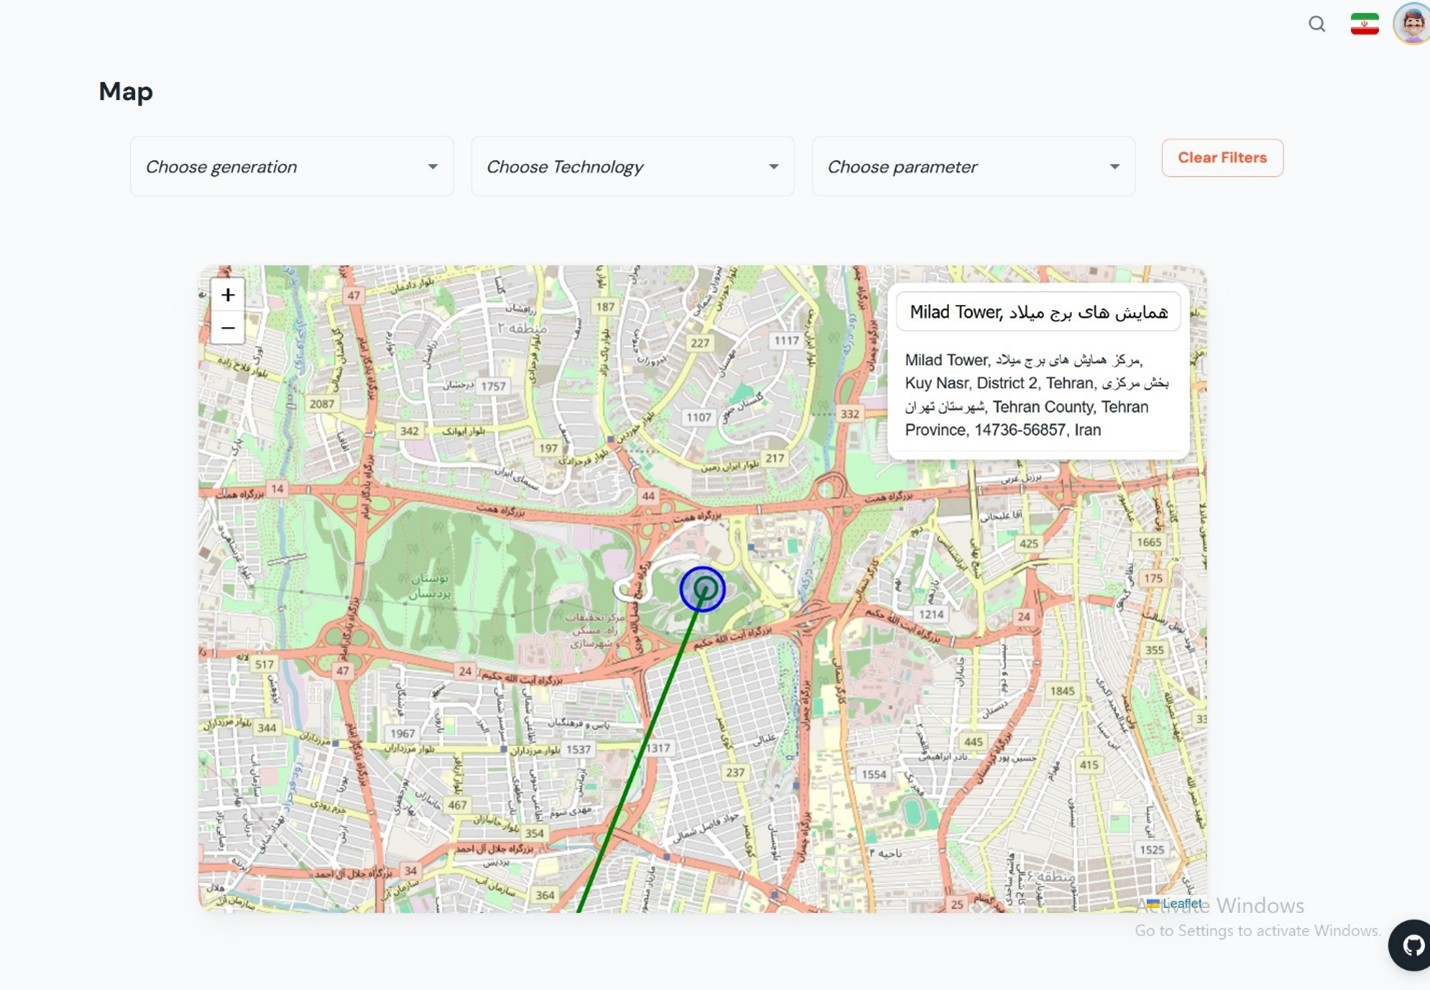
\includegraphics[width=0.7\textwidth,height=15cm,keepaspectratio]{Pic/map2}
		\label{fig:map2}
	\end{subfigure}\\*[5mm]
	\caption{تصاویر نقشه}
	\label{fig:mapsPic}
\end{figure}
\paragraph{توضیحات تکمیلی}
موقعیت جغرافیایی هر رکورد با یک دایره روی نقشه مشخص شده است. اگر روی آن هاور شود، یک تولتیپ نمایش داده می‌شود که تمامی اطلاعات شامل \textbf{آیدی سلول}, \textbf{نسل}, \textbf{تکنولوژی مورد استفاده} و \textbf{شاخص‌های کیفیت} مرتبط با آن تکنولوژی را نمایش می‌دهد. رنگ هر دایره نمایانگر کیفیت آن سیگنال است.
برای اینکه مسیر طی شده هنگام گرفتن تست روی نقشه نمایش داده شود، نقاط با خطوطی رنگی به هم وصل شده‌اند. اگر از یک نقطه با رنگ \textbf{a} به یک نقطه \textbf{y} با رنگ \textbf{b} برویم، رنگ خط میانی این دو نقطه برابر با رنگ نقطه شروع خواهد بود و می‌توانیم بفهمیم در مسیر تست، کیفیت بهبود یافته یا تضعیف شده است.
قابلیت فیلتر کردن نقاط روی نقشه بر اساس ویژگی یا ویژگی‌های دلخواه نیز وجود دارد که به تحلیل دقیق‌تر و سریع‌تر کاربر کمک می‌کند. همچنین می‌توانید از قابلیت سرچ مکانی که روی نقشه در اختیار شما قرار داده شده، بهره ببرید تا به یک نقطه مد نظر خود هدایت شوید.


\section{نوار پیمایش \lr{(Navigation bar)}}
در نوار بالای صفحه، برای تجربه بهتر شما، قابلیت‌های \textbf{سرچ}, \textbf{ست کردن پروفایل} و \textbf{انتخاب پرچم کشور} خود را دارید.

\begin{figure}[ht]
	\centering
	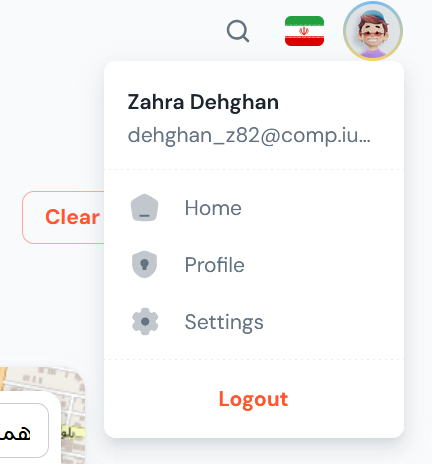
\includegraphics[height=5cm,keepaspectratio]{Pic/nav_menu}
	\caption{Navigation bar}
	\label{fig:nav}
\end{figure}

\section{اگر ادمین هستید بخوانید}
ادمین یک صفحه با نام \textbf{همه کاربران} دارد که می‌تواند پروفایل‌های همه کاربران فعال را ببیند. در صورت نیاز، ادمین می‌تواند وارد داشبورد آنها شده و مشکلات احتمالی را برطرف نماید.

\begin{figure}[ht]
	\centering
	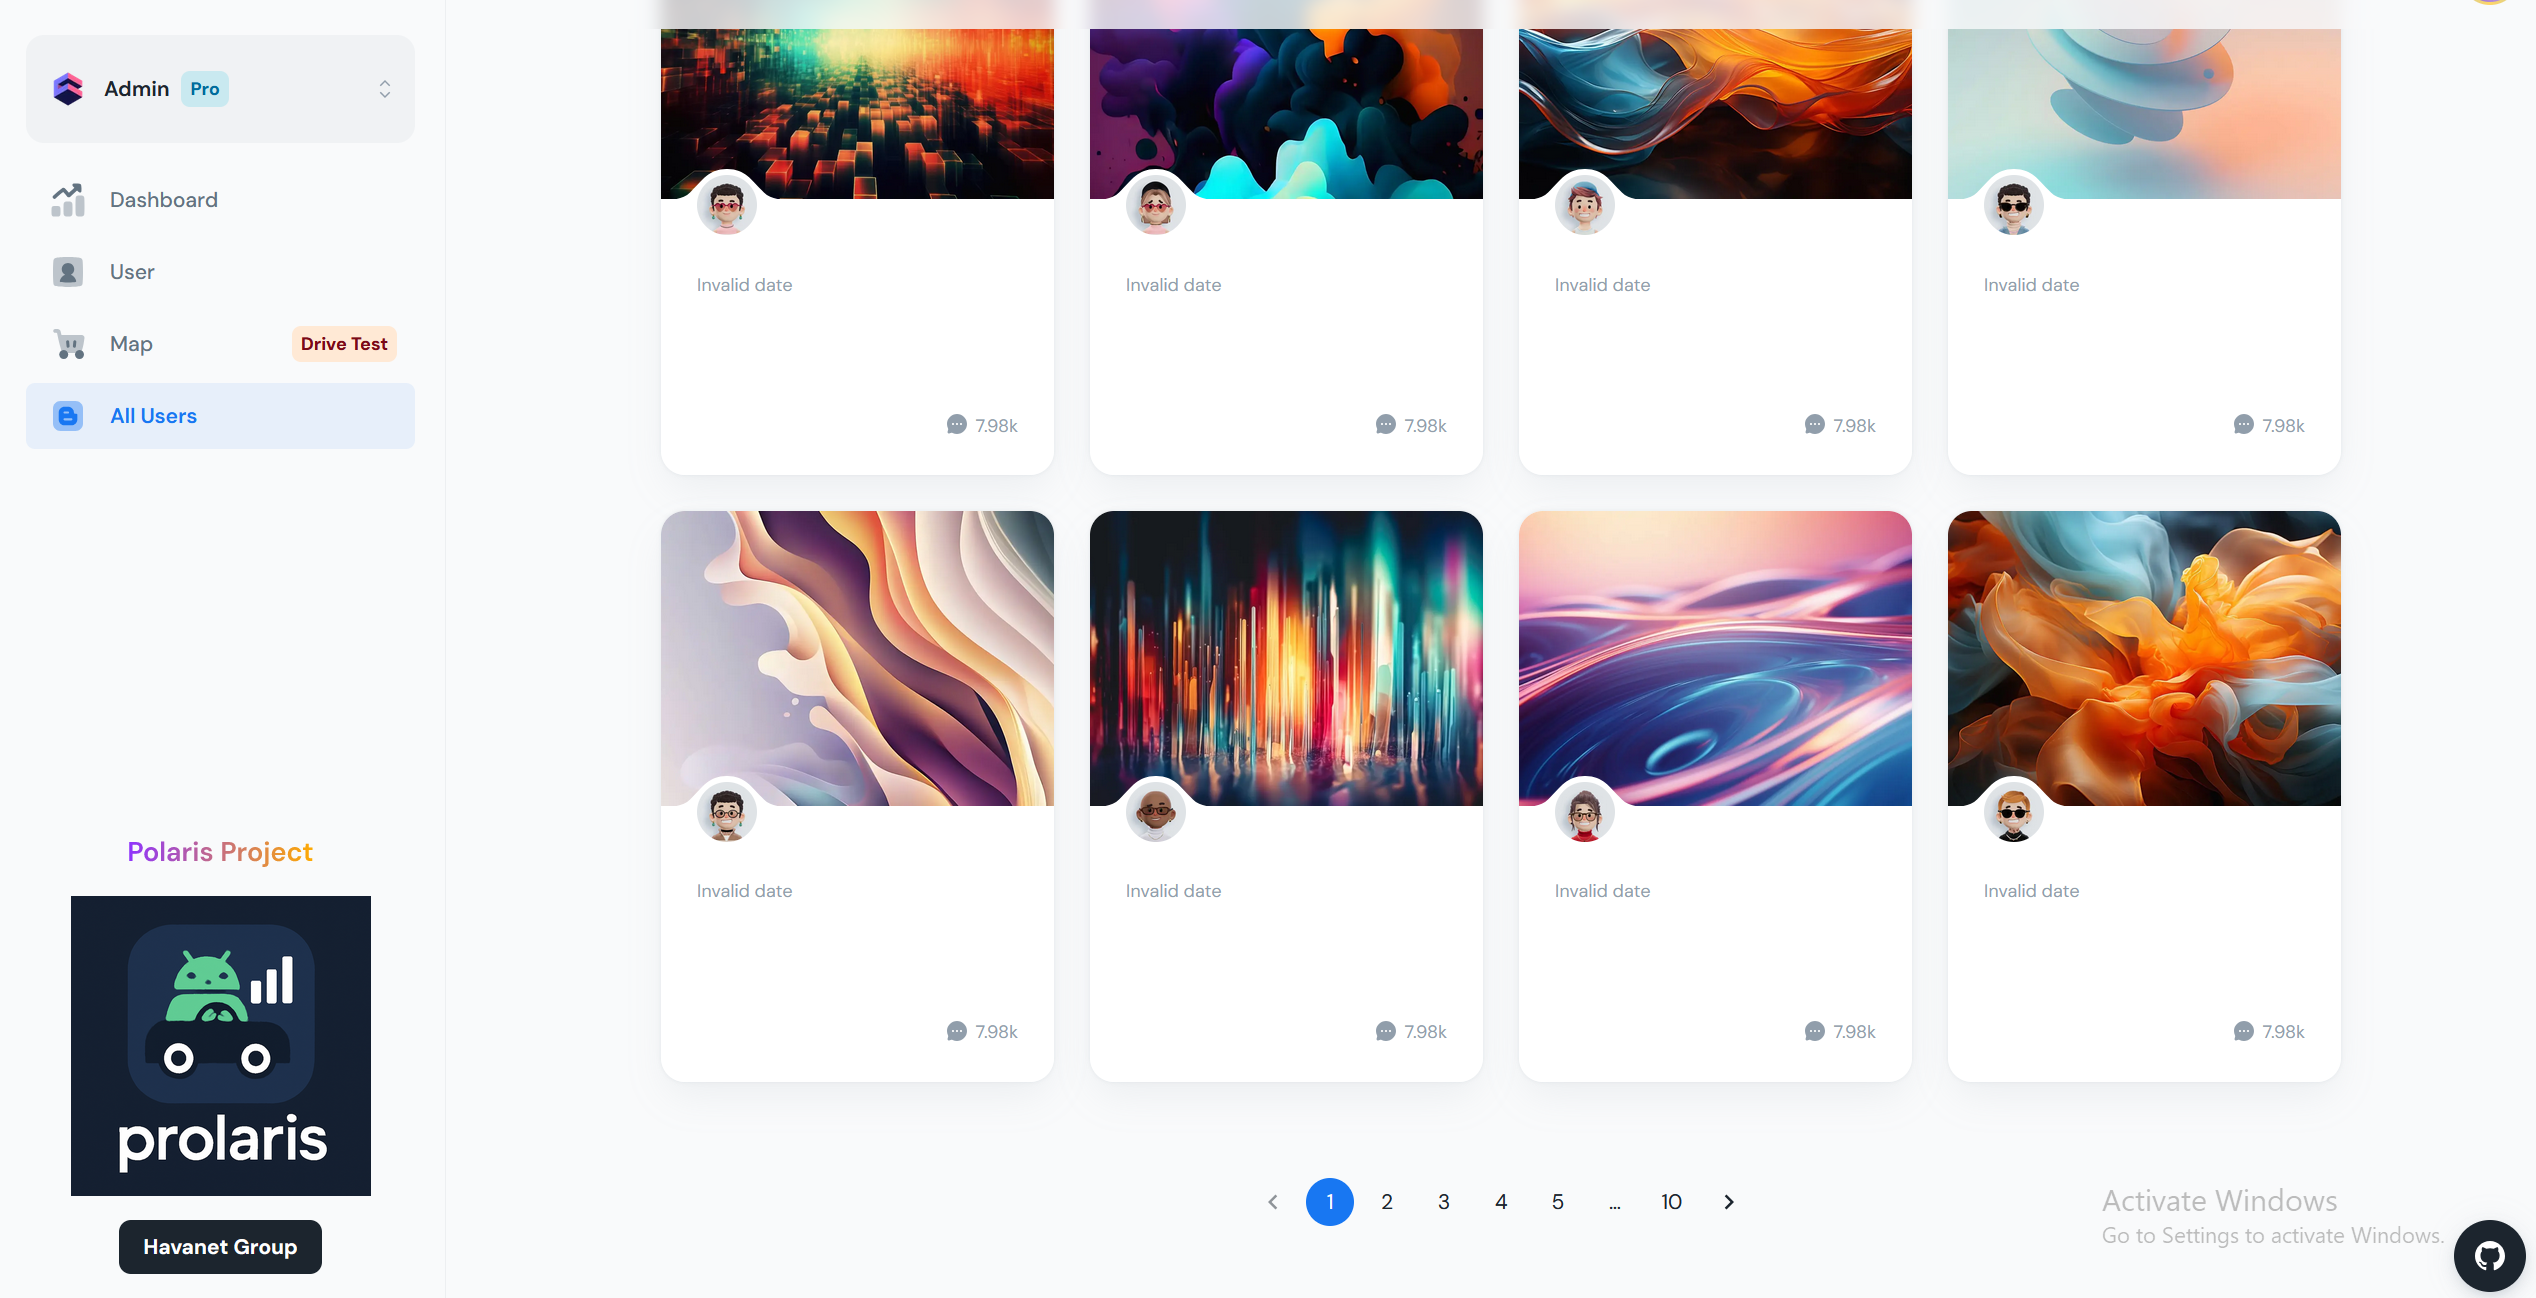
\includegraphics[width=0.7\textwidth,height=10cm,keepaspectratio]{Pic/admin}
	\caption{صفحه ادمین}
	\label{fig:admin}
\end{figure}

\chapter{ \lr{Android Mobile}}

\section{پیکربندی و راه‌اندازی اولیه اپلیکیشن}

برای اتصال اپلیکیشن به بک‌اند در محیط محلی، بک‌اند و موبایل باید در یک شبکه باشند. سپس آدرس IP سیستم میزبان بک‌اند را با دستور \textbf{ipconfig} در CMD پیدا کنید. آدرس \lr{IPv4} را یادداشت کرده و در محل زیر جایگزین کنید:

	مسیر: \\
	\begin{latin}
		\texttt{app/src/main/java/com/example/Havanet/viewmodels/SharedViewModel.kt}\\
	\end{latin}
	مقدار موجود در خط شماره پانزده، عبارت از:
\begin{latin}
\begin{lstlisting}[mathescape=true, numbers=left, firstnumber=15]
val ip = "10.13.148.180"
\end{lstlisting}
\end{latin}
	را با IP جدید جایگزین کنید.لطفاً دقت داشته باشید که پورت 8000 روی دستگاه شما باز باشد.

	

\vspace{0.5cm}

پس از انجام مراحل فوق، اپلیکیشن را با استفاده از \lr{Android Studio} روی دستگاه نصب کنید.

\section{مجوزهای موردنیاز}

اپلیکیشن برای عملکرد صحیح به مجوزهای مختلف نیاز دارد. برخی از این مجوزها هنگام اجرا از کاربر درخواست تأیید می‌شوند و باید آنها را قبول کند تا امکانات مربوط فعال شوند.

مجوزهای زیر هنگام اجرای برنامه از کاربر درخواست می‌شوند و باید حتماً اجازه داده شوند:

\begin{itemize}
	\item \lr{ACCESS\_FINE\_LOCATION}
	\item \lr{ACCESS\_COARSE\_LOCATION}
	\item \lr{READ\_PHONE\_STATE}
	\item \lr{SEND\_SMS}
	\item \lr{RECEIVE\_SMS}
\end{itemize}

سایر مجوزهای برنامه به صورت خودکار و بدون نیاز به تأیید کاربر فعال می‌شوند.

\section{صفحه ورود و ثبت‌نام}

پس از نصب و اجرای برنامه، صفحه \textbf{ورود/ثبت‌نام} نمایش داده می‌شود:
\begin{figure}[ht]
	\centering
	\begin{subfigure}[b]{0.3\textwidth}\centering
		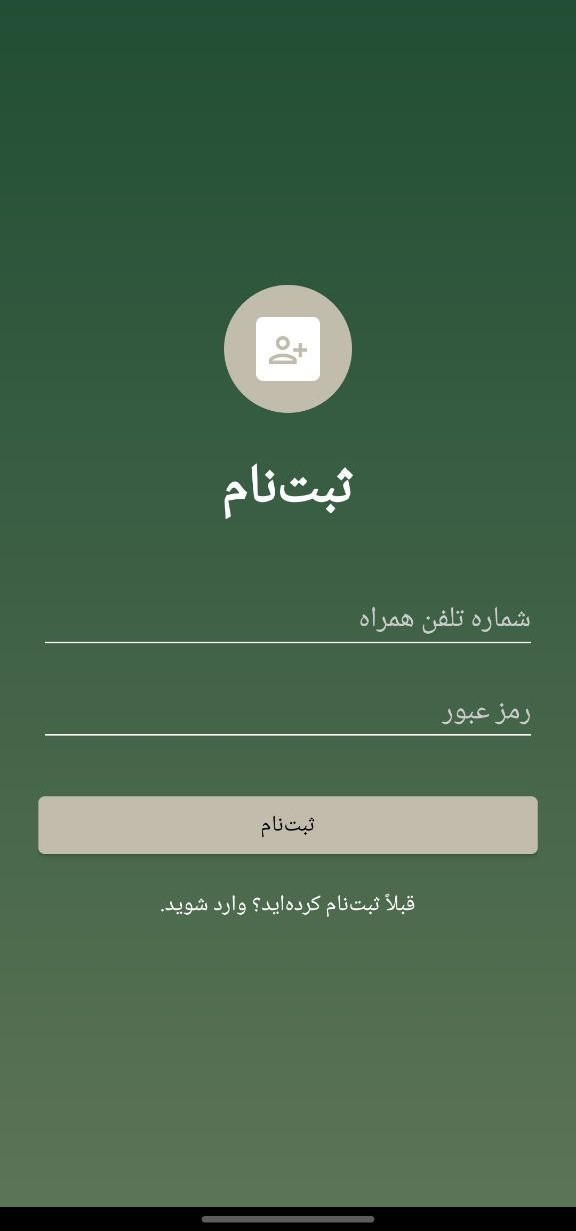
\includegraphics[width=0.7\textwidth,height=10cm,keepaspectratio]{Pic/signup}
		\caption{ثبت نام}
		\label{fig:signup}
	\end{subfigure}
	\begin{subfigure}[b]{0.3\textwidth}\centering
		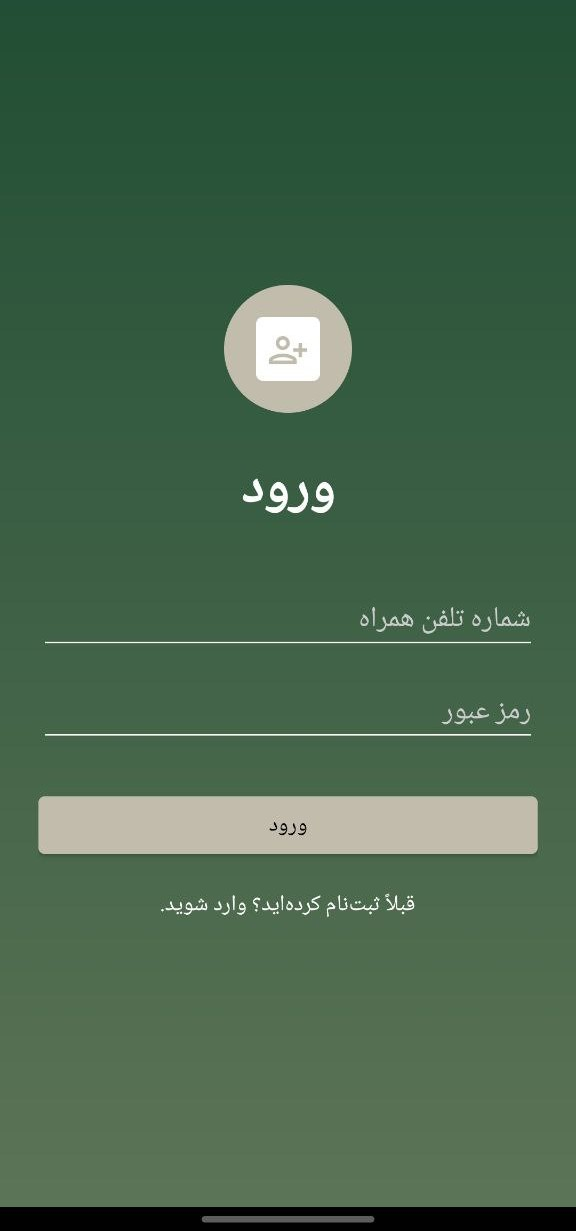
\includegraphics[width=0.7\textwidth,height=10cm,keepaspectratio]{Pic/login}
		\caption{ورود}
		\label{fig:login}
	\end{subfigure}
	\caption{اولین صفحات مشاهده شده}
	\label{fig:animals}
\end{figure}

\begin{itemize}
	\item \textbf{ثبت‌نام:}\\
	کاربر باید شماره تلفن همراه و رمز عبور خود را وارد کرده و اقدام به ایجاد حساب کاربری جدید نماید. رمز عبور باید حداقل شش کاراکتر داشته. درصورت داشتن اکانت، با لمس عبارت \textbf{«قبلاً ثبت‌نام کرده‌اید؟ وارد شوید.»} وارد صفحه ورود  شده.
	
	\item \textbf{ورود:}\\
	همانند صفحه ثبت نام با وارد کردن شماره تلفن همراه و رمزعبور وارد امانت خود شده. درصورت نداشتن اکانت، با لمس عبارت \textbf{«حساب ندارید؟ ثبت‌نام کنید.»} وارد صفحه ورود  شده.
\end{itemize}

\section{محیط اصلی}

\subsection{تنظیمات}

برنامه تنظیمات به شما امکان می‌دهد رنگ‌ها و مقادیر سطح مربوط به آن‌ها را برای نمایش داده‌های شبکه تنظیم کنید. 
این تنظیمات در سه مرحله اصلی انجام می‌شود: انتخاب گزینه‌ها، انتخاب رنگ‌ها، و ثبت نهایی. 

\begin{itemize}
	\item \textbf{انتخاب گزینه‌ها} \\
	در بالای صفحه، سه بخش برای انتخاب گزینه‌های اصلی وجود دارد:
	
	\begin{itemize}
		\item \textbf{تکنولوژی:} از منوی کشویی اول، نسل شبکه مورد نظر را انتخاب کنید. گزینه‌های موجود 2G، 3G، 4G و 5G هستند.
		\item \textbf{ویژگی:} با توجه به انتخاب شما در مرحله قبل، منوی کشویی دوم به‌روز می‌شود. این منو شامل انواع سیگنال‌های مربوط به تکنولوژی انتخابی است. به عنوان مثال، برای 4G، می‌توانید rsrp یا rsrq را انتخاب کنید.
		\item \textbf{تعداد رنگ‌ها:} از منوی کشویی سوم، تعداد سطوح مختلف کیفیت سیگنال را که می‌خواهید تعریف کنید، انتخاب کنید. این عدد بین 3 تا 50 قابل تغییر است و تعداد رنگ‌هایی را که باید به سیستم اضافه کنید، مشخص می‌کند.
	\end{itemize}
	\item \textbf{انتخاب و تعریف رنگ‌ها:}
	\begin{itemize}
		\item \textbf{انتخاب رنگ:} از چرخ رنگی بزرگ میانی استفاده کنید تا رنگ مورد نظر خود را برای یک سطح خاص از کیفیت سیگنال انتخاب کنید.
		\item \textbf{تعریف مقادیر:} پس از انتخاب رنگ، دکمه \textbf{افزودن رنگ} را فشار دهید. یک کادر گفت‌وگو ظاهر می‌شود که از شما می‌خواهد سه مقدار را وارد کنید:
		\begin{itemize}
			\item \textbf{عدد سطح:} عددی برای رتبه‌بندی کیفیت (مثلاً ۱ برای ضعیف، ۲ برای متوسط و ۳ برای خوب). هر رنگ باید یک عدد سطح یکتا داشته باشد.
			\item \textbf{حداقل مقدار بازه:} پایین‌ترین مقدار عددی برای این سطح کیفیت.
			\item \textbf{حداکثر مقدار بازه:} بالاترین مقدار عددی برای این سطح کیفیت.
		\end{itemize}
	\end{itemize}

	\item \textbf{ویرایش و نهایی کردن:}
	\begin{itemize}
		\item پس از افزودن هر رنگ، یک جعبه کوچک با رنگ انتخابی و عدد سطح آن در پایین چرخ رنگی نمایش داده می‌شود.
		\item برای ویرایش یک رنگ تعریف شده، روی جعبه رنگ مربوطه کلیک کنید. با این کار، رنگ در چرخ رنگی انتخاب می‌شود و می‌توانید با فشار مجدد دکمه \textbf{افزودن رنگ}، مقادیر آن را تغییر دهید. درصورت منصرف شدن از ویرایش با کلیک دوباره بر رنگ از حالت ویرایش خارج میشوید.
		\item زمانی که تعداد رنگ‌های انتخابی شما با عددی که در مرحله اول انتخاب کرده‌اید برابر شود، یک دکمه \textbf{ثبت نهایی} ظاهر می‌شود.
	\end{itemize}
	
	
\end{itemize}

\begin{figure}[ht]
	\centering
	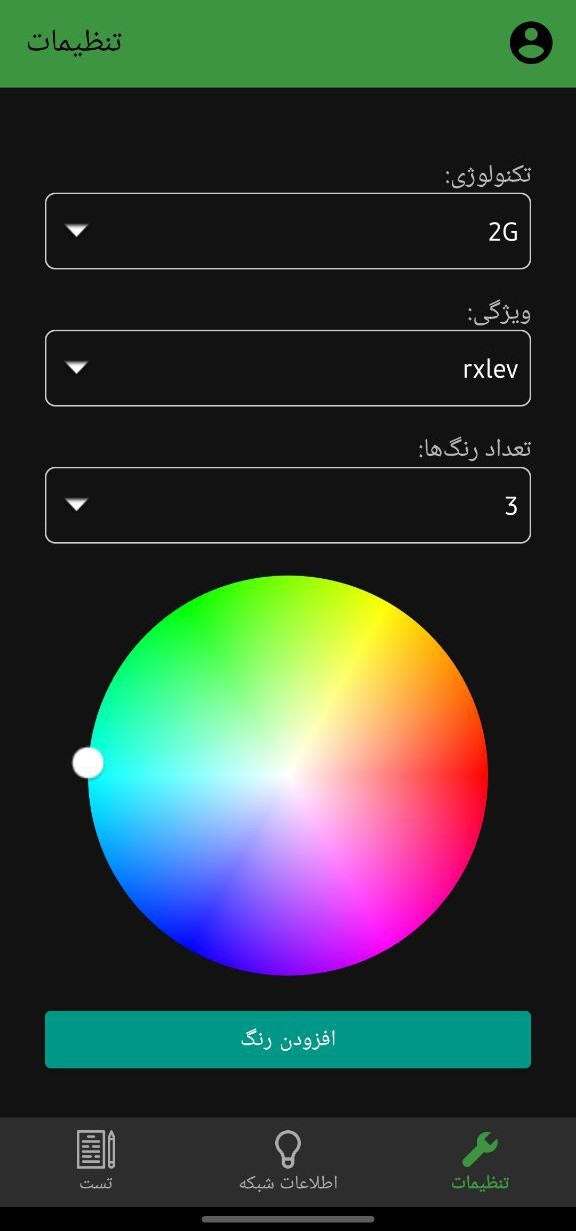
\includegraphics[width=0.7\textwidth,height=10cm,keepaspectratio]{Pic/setting}
	\caption{صفحه تنظیمات شبکه}
	\label{fig:setting}
\end{figure}

\subsection{اطلاعات شبکه}

در صفحه اطلاعات، وضعیت شبکه و موقعیت جغرافیایی کاربر به صورت زنده نمایش داده می‌شود.  
با فشردن دکمه \textbf{نمایش در نقشه}، موقعیت فعلی کاربر روی نقشه نشان داده می‌شود.

این اطلاعات به طور خودکار در پس‌زمینه به سرور ارسال می‌شوند و در همین صفحه می‌توان داده‌های ارسالی را مشاهده کرد.

\begin{figure}[ht]
	\centering
		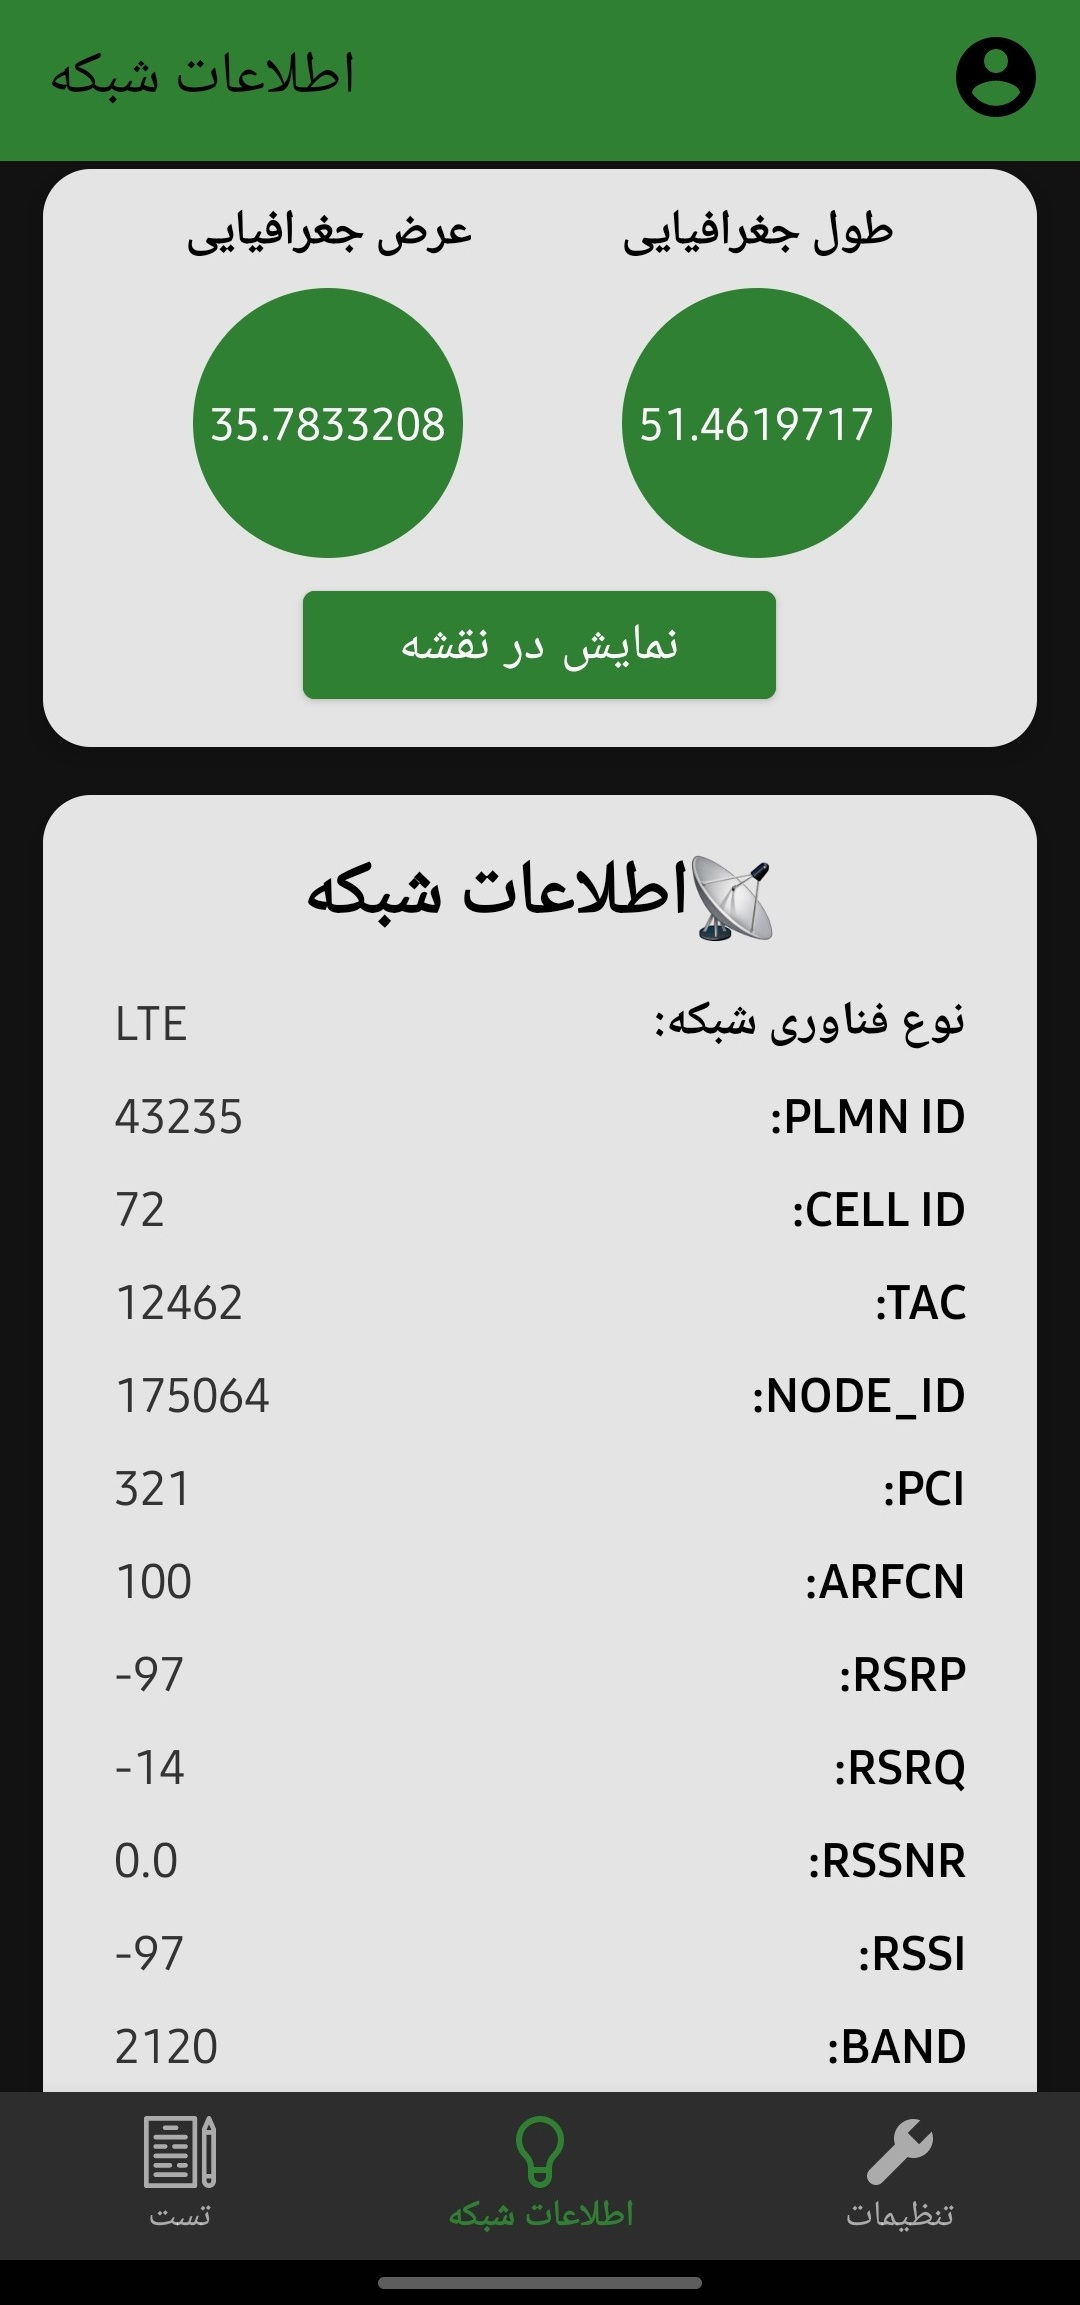
\includegraphics[width=0.7\textwidth,height=10cm,keepaspectratio]{Pic/info}
	\caption{صفحه اطلاعات شبکه}
	\label{fig:info}
\end{figure}

\subsection{تست‌ها}

با استفاده از این برنامه می‌توانید عملکرد و وضعیت شبکه اینترنت خود را با انجام تست‌های مختلف، به صورت دقیق بررسی کنید.

\begin{itemize}
	\item \textbf{بخش «تست‌های شبکه»} 

این بخش شامل شش دکمه برای انجام تست‌های مختلف شبکه است که می‌توانید به راحتی هر کدام را انتخاب و اجرا کنید.

\begin{itemize}
	\item \textbf{گذردهی دانلود (\lr{Download Throughput}):}\\
	با کلیک روی این دکمه، سرعت \textbf{دانلود داده} از سرور به گوشی شما سنجیده می‌شود. این تست برای ارزیابی عملکرد شبکه در هنگام دریافت فایل‌ها یا پخش ویدیو مفید است.
	
	\item \textbf{گذردهی آپلود (\lr{Upload Throughput}):}\\
	با کلیک روی این دکمه، سرعت \textbf{آپلود داده} از گوشی شما به سرور اندازه‌گیری می‌شود. این تست برای بررسی عملکرد شبکه در هنگام ارسال فایل‌ها یا آپلود تصاویر در شبکه‌های اجتماعی کاربرد دارد.
	
	\item \textbf{:Ping}\\
	این دکمه برای بررسی \textbf{زمان تأخیر (Latency)} در اتصال شبکه شما به یک سرور خاص به کار می‌رود. هرچه مقدار پینگ کمتر باشد، زمان پاسخ‌دهی شبکه بهتر است.
	
	\item \textbf{:DNS}\\
	این تست سرعت \textbf{پاسخ‌دهی سرور DNS} را می‌سنجد. DNS آدرس‌های وب ( \lr{www.google.com}) را به آدرس‌های IP ترجمه می‌کند. سرعت بالای پاسخ‌دهی DNS باعث لود شدن سریع‌تر صفحات وب می‌شود.
	
	\item \textbf{:Web}\\
	با کلیک روی این دکمه، عملکرد و سرعت \textbf{بارگذاری یک صفحه وب} مشخص تست می‌شود. این تست برای شبیه‌سازی تجربه واقعی کاربر هنگام مرور اینترنت طراحی شده است.
	
	\item \textbf{:SMS}\\
	این تست \textbf{سرعت ارسال پیامک (SMS)} را بررسی می‌کند. با این تست می‌توانید اطمینان حاصل کنید که سرویس پیامکی شما به درستی کار می‌کند.
	 \begin{figure}[ht]
		\centering
		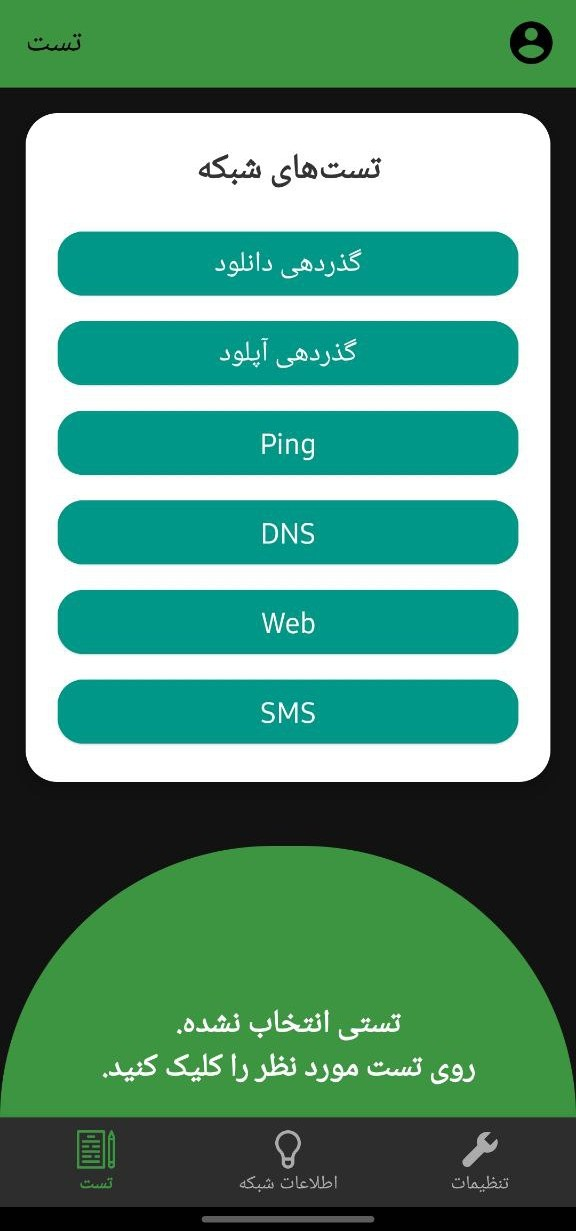
\includegraphics[width=0.7\textwidth,height=10cm,keepaspectratio]{Pic/test}
		\caption{صفحه تست ها}
		\label{fig:test}
	\end{figure}
\end{itemize}

\item \textbf{بخش «نتیجه تست»}  
در این بخش، نتایج تست‌های اجراشده نمایش داده می‌شود.\\
پیش از شروع هر تست، پیامی ظاهر می‌شود که از شما می‌خواهد روی دکمه موردنظر کلیک کنید.\\
هر تست در بازه‌ای دو دقیقه‌ای اجرا می‌شود و بین مراحل آن تأخیری ۱۰ ثانیه‌ای وجود دارد. 
به همین دلیل، پس از شروع یک تست، سایر دکمه‌ها تا پایان زمان دو دقیقه غیرفعال خواهند بود.\\

همچنین توجه داشته باشید که اگر هنگام اجرای تست از صفحه خارج شوید، فرآیند تست ناتمام باقی خواهد ماند.
\end{itemize}

\subsection{مدیریت حساب کاربری}

این صفحه به شما امکان می‌دهد اطلاعات حساب کاربری خود را مشاهده و مدیریت کنید.

\begin{itemize}
	\item \textbf{مشاهده و ویرایش اطلاعات حساب:}  
	در بخش میانی صفحه، سه فیلد برای نمایش اطلاعات شما وجود دارد:
	\begin{itemize}
		\item \textbf{شماره تلفن همراه:} شماره تلفن همراه کنونی، که با آن ثبت نام کرده اید را نشان می دهد.
		\item \textbf{رمز عبور:} رمز عبور شما به صورت محرمانه و با ستاره نمایش داده می‌شود.
		\item \textbf{نقش:} یکی از دو نقش "کاربر" یا " ادمین نشان که نشان دهنده دسترسی های شما هست.
	\end{itemize}
	
	\item \textbf{خروج از حساب:}  
	در پایین صفحه، یک دکمه با عنوان \textbf{«خروج»} وجود دارد. با ضربه زدن روی این دکمه، شما از حساب کاربری خود خارج خواهید شد.
\end{itemize}

 
  \begin{figure}[ht]
 	\centering
 	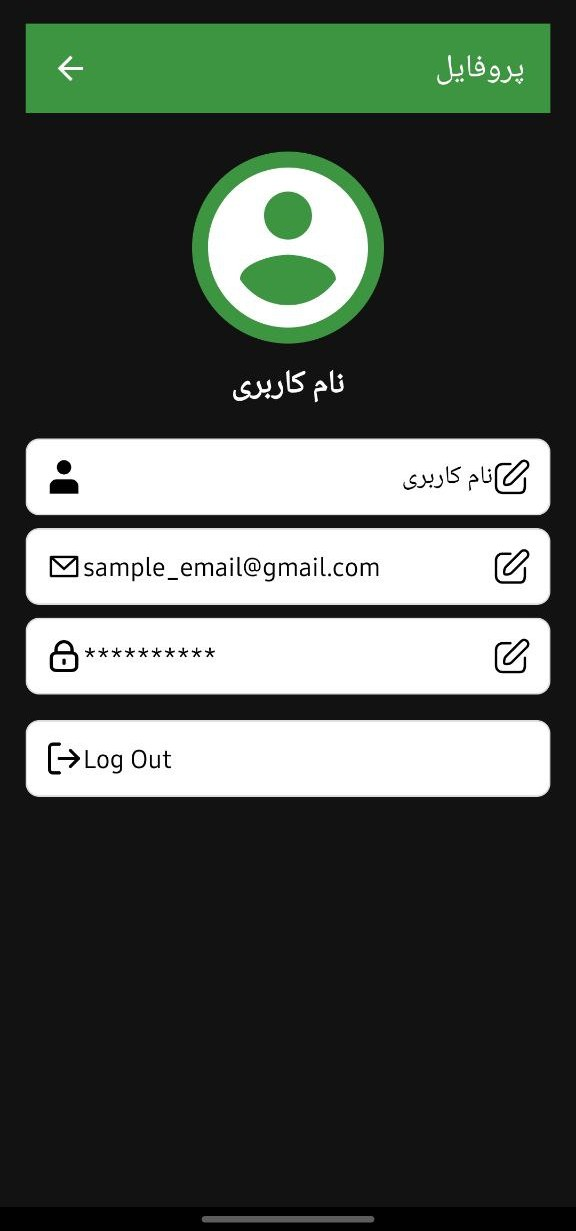
\includegraphics[width=0.7\textwidth,height=10cm,keepaspectratio]{Pic/profile}
 	\caption{صفحه حساب کاربری}
 	\label{fig:profile}
 \end{figure}
\end{document}



